%!Tex Root = ../Tutorat6.tex
% ./Packete.tex
% ./Design.tex
% ./Deklarationen.tex
% ./Aufgabe1.tex

\section{Task 2}

\setcounter{task}{1}
\begin{frame}{Task 2}{Design space exploration}
    \begin{tasknoinc}
        Consider again the sequence graph and the specification of task 1. Assume that there is only one resource type which can compute all operations $(+, -, <, *)$ and has an area of 1. The cost of an implementation is given by the total required area. The goal is to find the Pareto-points of the design space which is given by the parameters cost and latency. The number of allocated resources is not yet fixed.
        \bigskip

        Compute a lower and an upper bound for the latency in order to limit the possible Pareto-points.
    \end{tasknoinc}
\end{frame}
\begin{frame}{Task 2}{Design Space Exploration}
    \begin{solution}
        \begin{itemize}
            \item The latency bounds are easily determined by considering the sequence graph of exercise 1.
            \item We have seen, that we can achieve a Latency of $L = 11$ with just one resource. Hence $L \leq 11$.
            \item We have also seen that with an unlimited amount of resources, the best we can achieve is $L = 4$ since the dependencies won't allow us to go any faster, no matter how many ressources we can use to distribute operations on. Hence $L \geq 4$
            \item Thus, the bounds for $L$ are: $4 \leq L \leq 11$
        \end{itemize}
    \end{solution}
\end{frame}
\begin{frame}{Task 2}{Design space exploration}
    \begin{tasknoinc}
        Compute a lower and an upper bound for the cost in order to limit the possible Pareto-points.
    \end{tasknoinc}
\end{frame}
\begin{frame}{Task 2}{Design Space Exploration}
    \begin{solution}
        \begin{itemize}
            \item The costs are determined by the area, that is, in this case, the amount of resources we use. Our lower and upper bound for $L$ helps us to find the bounds for $c$ more quickly.
            \item In the slowest case, we had $L = 11$ with just one resource, hence $c \geq 1$
            \item In the fastest case, we had $L = 4$ with unlimited resources. What finite number of resources are necessary, to achieve the same latency?
            \item [$\Rightarrow$] An easy to see upper bound to reach the lowest latency is $c = 5$. However, it's possible to reduce the resources even further to obtain $c \leq 3$.
        \end{itemize}
    \end{solution}
\end{frame}
\begin{frame}{Task 2}{Design space exploration}
    \begin{tasknoinc}
        Find all Pareto-points and represent them in a diagram.
    \end{tasknoinc}
\end{frame}
\begin{frame}{Task 2}{Design space exploration}
    \begin{solutionnoinc}
        \begin{itemize}
            \item First we have to consider the set of all possible solutions $(L, c)$. Our lower and upper bounds help us to vastly reduce the amount of solutions that we have to consider.
            \item For each c $\in \{1, 2, 3\}$ we determine the fitting latency L and obtain:
            \item [] Solution 1: $(11, 1)$
            \item [] Solution 2: $(6, 2)$
            \item [] Solution 3: $(4, 3)$
            \item Out of these solutions, we now determine the Pareto-optimal front.
        \end{itemize}
    \end{solutionnoinc}
\end{frame}
\begin{frame}{Task 2}{Design space exploration}
    \begin{requirementsnoinc}
     A solution $a \in X$ weakly Pareto-dominates a solution $b \in X$ denoted as $a \preceq b$, if it is as least as good in all objectives, i.e. $f_i(a) \leq f_i(b)$ for all $1 \leq i \leq n$. Solution a is \alert{better} than b, denoted as $a \prec b$, iff $(a \preceq b) \land (b \npreceq a)$.
    \end{requirementsnoinc}
    \begin{solutionnoinc}
        \begin{itemize}
            \item Looking at out three solutions $(11, 1), (6, 2), (4, 3)$ it is clear that according to the above definition, no solution is \alert{better} than the other. Meaning, we already have found the Pareto-optimal front!
        \end{itemize}
    \end{solutionnoinc}
\end{frame}
\begin{frame}{Task 2}{Design space exploration}
    \begin{solution}
     \begin{figure}
         \centering
         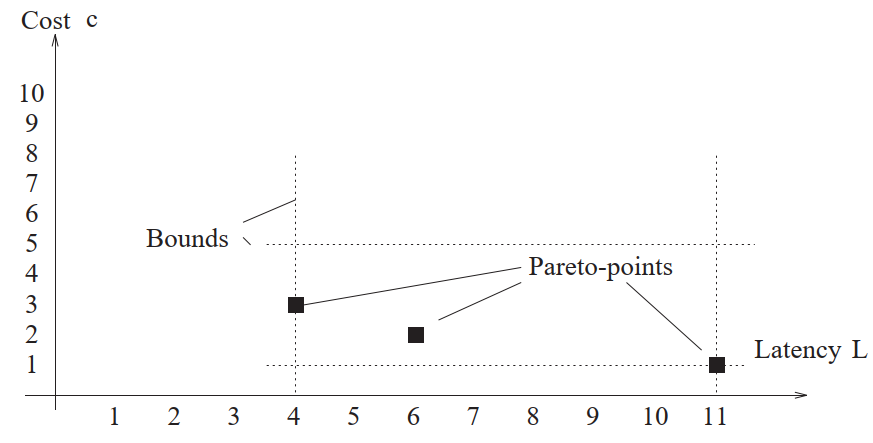
\includegraphics[scale=0.3]{figures/Pareto-points.PNG}
         \caption{Pareto-points}
     \end{figure}
    \end{solution}
\end{frame}
\begin{frame}{Task 2}{Design space exploration}
    \begin{Sidenote}
    If we had chosen $1 \leq c \leq 5$, the solutions would have been $(11, 1), (6, 2), (4, 3), (4, 4), (4,5)$. It is obvious, that $(4, 3) \preceq (4, 4)$ and $(4, 3) \preceq (4, 5)$ but not the other way around. Hence the last two solutions are inferior compared to $(4, 3)$ and can be removed from the set of solutions. As conclusion, finding a tighter bound helps us to immediately reduce the solution space we have to explore. Though, it might not always be so easy to find these bounds in the general case.
    \end{Sidenote}
\end{frame}
